\chapter{figo GmbH}
\label{chaper:figo}
The German banking system is divided into three large sectors: private, public, and cooperative. The cooperative sector is represented by 1,144 credit unions and 2 cooperative central banks. The public sector employs 431 savings bank, 10 land banks and other institutions. Private banks represented 4 transnational banks, 42 investment banks, and 176 regional and other banks. There is also operating are 167 registered branches of foreign banks, including 60 investment banks\cite{listOfBanks}.   

The introduction of Payment Services Directive (PSD) and PSD2 by European Commission in EU together with initiatives of UK Government regarding API provision and standardization have obligated banks with the implementation of on-line access points to their services\cite{LarsAPI}\cite{TimAPI}\cite{DaveAPI}. Within the Single European Payment Area acceptance of directive by European Bank Authority scheduled within 2017 year\cite{PSD2}.

figo GmbH is a financial technology (FinTech) company with the headquarter located Hamburg, Germany. It was founded in 2012  with the mission “to build the backbone of next generation financial services"\cite{figoFAQVision}.  Currently, the API is fully functional in Germany, partly in Austria and England\cite{figoAngel}\cite{figoCB}.

figo Connect API was created with the aim to accelerate innovations in the FinTech area and to allow figo's partners to offer products with real added value\cite{figoFAQWhat}. It enables developers, startups, and even banks to connect to every financial service. These partners can access every bank account (current, savings, loan, securities, etc), credit card, eWallet and other financial services l(i.e. PayPal) through one single REST-API \cite{figoFAQWhat}\cite{figoFAQVision}\cite{figoFAQPartners}. The list of figo's partners and customers  together with their use cases can be found via following link: \url{http://figo.io/use\_cases.html}.


%"The Figo GmbH was founded in 2012 and has its headquarters in Hamburg.
%Figo is a modern and safe with the Figo Connect banking as a service ready platform. Developers can integrate into a variety of services and services thanks to Figo very easy and fast online banking. In addition to the retrieval of account balances and transactions in almost all banks, credit cards and services like PayPal, payments on the platform can be initiated. Figo operates the platform in a German bank for the data center and has been with the "Cloud Services Made in Germany awarded" seal."\cite{figoFAQWhat}
%"The current development in the FinTech scene just shows the need for innovation in the field of finance. Too much was thought of in silos in recent years, and products / services have been developed over the customer. This trend reverses itself just around, and we Figo strive in the same direction. For this reason, we have the Figo Connect API in order to accelerate innovation in the FinTech area and want to allow our partners to offer products with real added value."\cite{figoFAQVision}\\
%"Figo is working with a variety of partners. These partners use our API for very different purposes. "\cite{figoFAQPartners}.List of partners of Figo API with their usecases 
%http://figo.io/use\_ cases.html\\

%"figo’s mission is to “build the backbone of next generation financial services”. 

%Our banking API enables developers, startups and even banks to connect to every financial service provider. These partners can access every bank account (current, savings, loan, securities, ...), credit card, eWallet and other financial services through one single REST-API. It is possible to extract account information and initiate bank transfers \& direct debits.
%With our API, old and new players of the financial service industry are able to easily develop and test new services without the inconvenience of connecting to every single bank.

%Currently, the API is fully functional in Germany and partly in Austria (more countries to follow). Please contact us for access to our API."\cite{figoAngel}

%"Our banking API enables developers, startups and even banks to connect to every financial service provider. These partners can access every bank account (current, savings, loan, securities, ...), credit card, eWallet and other financial services through one single REST-API. It is possible to extract account information and initiate bank transfers \& direct debits. With our API, old and new players of the financial service industry are able to easily develop and test new services without the inconvenience of connecting to every single bank."\cite{figoCB}

\section{IT infrastructure. Banking Server}
\label{sec:infrastructure}
The high-level IT infrastructure of figo GmbH consists two parts (Fig. \ref{fig:figoArch}). The \textbf{API Server} implements interfaces to figo's customers and partners for accessing banking information and services (lays outside of the paper's scope). The \textbf{Banking Server} implements the connections to banks via three possible communication channels, their description provided below together with basic motivation for each of them.
\begin{figure}[ht]
  	\label{fig:figoArch}
    \centering
    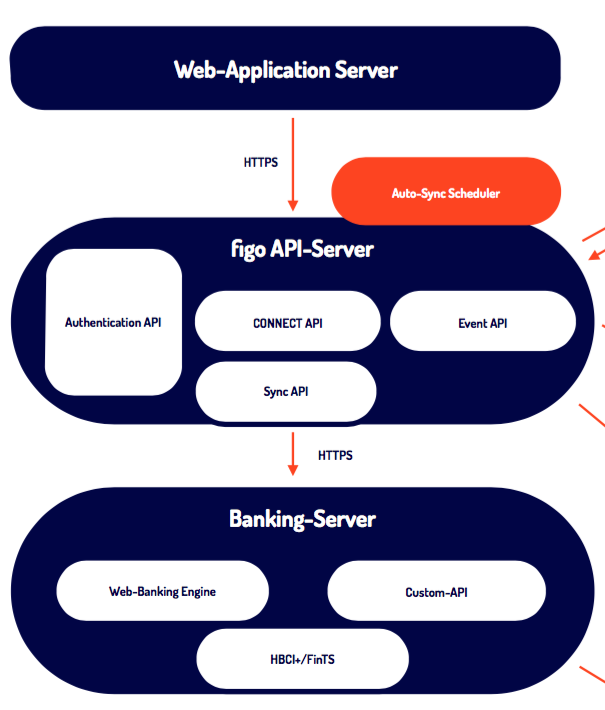
\includegraphics[scale=0.7]{grafiken/figoArch}
     \caption{figo GmbH high level architecture}
\end{figure}

\subsection{Banking Server Architecture}
\label{sec:bankingArch}
	Banking server has three parts for communication with banks via three separate channels. Each of them is a realization of different technology in a same programming language - javascript.  

	\paragraph{Custom-API} is responsible for connection to custom APIs provided by banks. It implements the client for custom banks APIs. Some of them provide full functionality while some only partial. All this APIs vary in their structure and functionality but most of them  are an implementation of REST-API specification.
	
	\paragraph{HBCI+/FinTS} is responsible for connection to banks' interfaces via Home Banking Computer Interface (HBCI). It is an implementation of an \textit{adapter OOP pattern} for the jsHBCI library.  HBCI is an open publicly available protocol. Its specification was originally designed by the two German banking groups \textit{Sparkasse and Volksbanken und Raiffeisenbanken} and \textit{German higher-level associations as the Bundesverband deutscher Banken e.V.}.  \cite{finTS}
	
	\paragraph{Web-Banking Engine} is responsible for communication with banks which does not provide API or HBCI. This is an implementation of a \textit{factory OOP pattern} for scraping libraries. Here figo GmbH uses \textit{web scraping} technology to perform interaction with internet-banking web pages.
	From the banks perspective, the interaction looks completely like direct communication with an user, while a user does not feel the difference between interaction via Custom-API or HBCI or Web-Banking Engine while accessing his bank or service via figo API.
	This is the most sensitive part from the developer's perspective since every change to the bank's web page can lead to failure of the specific scripts. \\
	
%	The aim of this paper is an application of Test Sheet for early (before any user's interaction will take place) recognition of page changes  and notification of developers regarding failed part of the script.
	
	%\subsection{Banking Technology Stack}
	%banking server only
	
%and analyses the difference in requirements differences defined by Test Sheets concept and introduced by figo GmbH.

%Firstly the platform of the implementation must be node.js its conceptual differences with such enterprise languages as Java or C# can be understood from the paltform description provided earlier in this paper but it worth to highlight them explicitly. The language of implementation is javascript which is the language with \textit{prototype based inheritance}. The \textit{event-loop mechanism} placed in core of the platform makes it asynchronous. Support of f\textit{unctions as a first-class citizens} provides an ability of confrontational function passing which is a pattern of functional programming. The language is relatively new for implementation of server-side applications.



%Test Sheets were originally designed for test definitions of OOP languages. And all available examples describes tests definitions for Java Classes. While figo GmbH case requires implementation of tests for nodeJS/casperJS, which are based on JavaScript - Object Oriented, imperative, Functional Oriented programming language with asynchronous information flow.
%Moreover figo GmbH requires input of test results to be recorded in to LogStash logs database. 

%Testing of real-time software


%The execution requirements from figo GmbH are such that tests defined via Test Sheets should be automatically executed in a time manner (every 2 mins or so), while normal software testing is performed on demand.
%The figo's requirement for comparison is such that while defining a Test Sheet user should be able to select from two types of comparison: 1) Strict comparison - complete comparison of objects including both properties' structure and their values. 2) Not-Strict comparison - scheme comparison of objects.

%(Probably should go to different section)
%Scraping scripts implement callback based approach for handling asynchronous data flow. This provides an opportunity to perform result comparison within the custom callback defined on a implementation stage.
%Standard convention for callback definitions limitates number of input parameters of a callback (error, data), while comparison requires compare data parameter with expected outputs from Test Sheet. The opportunity to resolve this issue lays in a JavaScript's support of functions as a class citizens, the function implementation of module for comparison and report: module exports function which invoked with single parameters (expected\_output) / ( + script name) and returns function which is used as a callback for scrapping script, this callback function performs comparison and writes its result to TestSheet or logstash depending on environment in which the program was executed


%%!!! update conventions and align this list to them!
%\begin{enumerate}
%	\item asynchronous software in combination with reference mechanism of test sheets
%\end{enumerate}

\section{Transformation project}
\label{sec:transP}
This section describes transformation project created by figo GmbH for use of Test Sheets within the organization.
\textbf{Enterprise System Transformation} -  "is a hierarchic-sequential process involving all actions of individuals in an organization leveraging information technology to support the transition of an Enterprise System from its original O-I-T[(Fir.:\ref{fig:oit})] configuration [...] to an (enhanced) O-I-T[(Fir.:\ref{fig:oit})] configuration."\cite{MES5}

\begin{figure}[ht]
	\label{fig:oit}
	\centering
	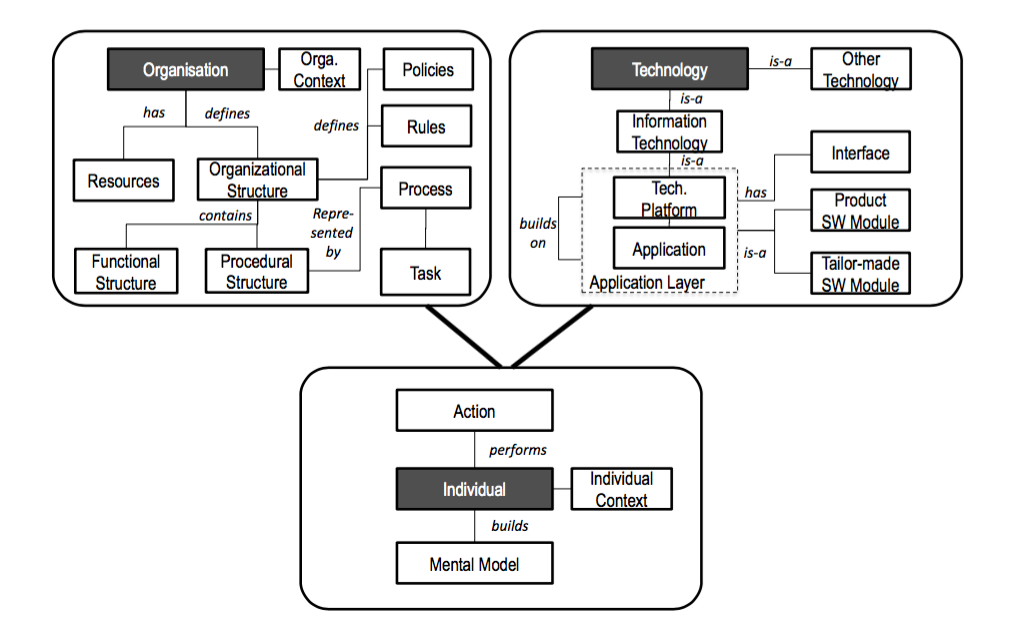
\includegraphics[width=\textwidth]{grafiken/oit.png}
	\caption{O-I-T model\cite{MES5}}
\end{figure}

The transformation project includes within itself four processes:
\paragraph{Development} focuses on the issue how information systems are developed. In contrast to software engineering, software development takes the socio-technical perspective on information systems\cite{MES6}.

\paragraph{Adoption} is a process defined by three concepts\cite{MES7}
\begin{enumerate}
	\item \textbf{Diffusion} refers to the breadth of use, e.g.the number of adopters in an organization
	\item \textbf{Infusion} describes how extensively the technology is used and the level of impact within the organization
	\item \textbf{Assimilation} addresses how extensively the new technology is used and how deeply the firm's use of the technology alters processes, structures, and organizational culture
\end{enumerate}

\paragraph{Convertion} is a process of realization of transformation projects with goal of successful system transformations \cite{MES9}

\paragraph{Use} continues process closely coupled with conversion process. It covers not only the process of the system usage by the individuals but also the impact of it on the organization in context of short- and long-term benefits. Individuals in the context of their performance and satisfaction.

\subsection{Test Sheets project}



%The tool should provide business staff of the company to define business scenarios in a non-technical way. After definition such scenarios must be executed over web-page. Create, Read, Update, Delete (CRUD) operations for this scenarios must be performed with .

\paragraph{Project definition:} Introduction of a tool for verification and/or testing of product’s functional fit to its requirements (i. e. detection of changes in banks web-pages, local software failures and/or errors) with minimal involvement of software developers into the process. Continuous project which requires software to be developed and supported by developers and can be executed on workstations of product/project managers.

\paragraph{Project uncertainties:}
\begin{itemize}
	\item Priority
	\item Functional fit
	\item Maintenance process
	\item Functionality enhancement
	\item Organizational culture fit
\end{itemize}

\paragraph{Rationale for project creation and focus.} 
\begin{itemize}
	\item High workload and time pressure in combination with limited technical resources leads to less time available on manual system monitoring. Non developers were not capable of testing the functionality;
	\item Tests will help in estimation of time to fix errors.
\end{itemize}


\paragraph{Underlying assumptions.} Shift of responsibility for functionality  on managers will improve system maintenance process and customers' user experience. 

\paragraph{Goal.} Routinization of product verification/testing process with respect to its business and functionality requirements by use of Test Sheets.
\paragraph{Plan:}
\begin{itemize}
	\item Test Sheets concept introduction to the target customers
	\item Requirements analysis 
	\item Mapping requirements to the concept of Test Sheets
	\item Dfinition of the development process
	\item System design
	\item Development:
	\begin{itemize}
		\item Alpha1 version without support of references and optimization for real-time testing
		\item Alpha2 version with references support and optimization for real-time testing
		\item BETA version with optimization for real-time testing
		\item Reporting mechanism
	\end{itemize}
	\item Demonstration
	\item Performance measurements
	\item Workshop on system installation and usage
	\item Routinization
	\item UX collection
\end{itemize}

\paragraph{Success:}
\begin{itemize}
	\item Goals are met;
	\item The system is fully routinized within the business processes;
	\item The time for bugs allocation and fix is reduced;
	\item The number of affected customers is minimized.
\end{itemize}


\subsection{Technical requirements}
First, test execution must be performed in a timely fashion for an opportunity to detect changes as early as possible to prevent attempts of customers' communication with not available banks or services. Consequently, tests execution have to be fast. 
Nextm software developers must be notified about script failure as soon as it was detected to improve response time. 
Moreover, scraping scripts are communicating with web-pages in a real-time and asynchronous fashion. 
Further, the language of implementation must be javascript for low entry level of developers in the future maintenance process. 
Last but not least, due to the nature of data represented on a web page the comparison between actual and expected results must have two possible options: object keys comparison and object key-value comparison.


